\def\currentRootFolder{chapter/sensitivityStudyWithPreliminaryKatrinElossModel/statisticalPrerequisites}
\def\currentFigureFolder{\currentRootFolder/fig}
\newcommand{\elecIndex}{\mathrm{e}}

\newcommand{\Bsource}{B^j_\mathrm{S}}
\newcommand{\BsourceAvg}{B_\mathrm{S}}
\newcommand{\zSource}{z_\mathrm{S}}
\newcommand{\thetaSource}{\theta_\mathrm{S}}
\newcommand{\thetaSourceAvg}{\theta_\mathrm{S}}
\newcommand{\Esource}{E_\mathrm{S}}
\newcommand{\Usource}{U^j_\mathrm{S}}
\newcommand{\gammaSource}{\gamma_\mathrm{S}}


\newcommand{\Bps}{B_\mathrm{PS2}}
\newcommand{\Bana}{B_\mathrm{A}}
\newcommand{\Bpinch}{B_\mathrm{P}}
\newcommand{\Bmax}{B_\mathrm{max}}
\newcommand{\Bmin}{B_\mathrm{min}}

\newcommand{\thetaMax}{\theta_\mathrm{max}}
\newcommand{\Esur}{E_\mathrm{sur}}
\newcommand{\detEff}{\epsilon_\mathrm{det}}
\newcommand{\macefilterwidth}{\Delta \mathcal{E}^j(\thetaS^j)}

\newcommand{\EtransPure}{E^j_\mathrm{tr}}
\newcommand{\Etrans}{\EtransPure(qU,\Esource,\thetaSource)}
\newcommand{\thetaTransPure}{\theta^j_\mathrm{tr}}
\newcommand{\thetaTrans}{\thetaTransPure(\Esource,qU)}

\newcommand{\As}{A_\mathrm{S}}
\newcommand{\Rbg}{R_\mathrm{bg}}


\newacronym{standardmodel}{SM}{Standard Model of Particle Physics}
\newacronym{lep}{LEP}{Large Electron Positron Collider}
\newacronym{ssm}{SSM}{standard solar model}

\section{Statistical Prerequisites}
\label{sec:katrinElossStatistics}
This section develops the statistical tools used in the scope of this thesis in order to evaluate the impact of the KATRIN model on KATRIN's sensitivity to the neutrino mass. The methods are described in a general manner (and could be applied to study model uncertainties in general) and then related to the KATRIN model. Section~\ref{sec:katrinElossStatisticsCombMeasurements} presents a concept for a combined parameter inference based on multiple measurements. Section~\ref{sec:katrinElossStatisticsProfileLikelihood} introduces the profile likelihood method for the treatment of nuisance parameters. And section~\ref{sec:katrinElossStatisticsImplementation} outlines how the statistical concepts were implemented into the KaFit (see section~\ref{sec:statMethodsKaFitSSC}) software framework.

\subsection{Combination of Commissioning and Neutrino Mass Measurements}
\label{sec:katrinElossStatisticsCombMeasurements}
\begin{figure}[t]
	\centering
	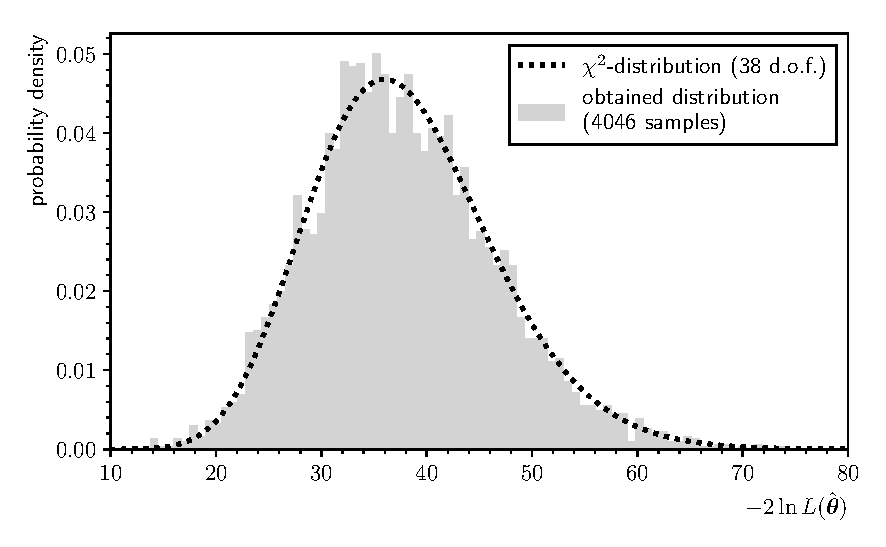
\includegraphics[width=\textwidth]{\currentFigureFolder/katrinElossChi2Distribution.pdf}
	\xcaption{}{}{}
	\label{fig:katrinElossStatisticsChi2}
\end{figure}


If two measurements share a set of parameters $\paramVecShared$, but have additionally an individual set of parameters $\paramVec_1$ and $\paramVec_2$ and different sets of observations a combined likelihood is given by the product of the single likelihoods $L_1$ and $L_2$
\begin{equation}
-2\ln L(\paramVecShared, \paramVec_1, \paramVec_2) =  
-2\ln L_1(\paramVecShared, \paramVec_1)
-2\ln L_2(\paramVecShared, \paramVec_2)
\fullstop
\end{equation}
In the case of KATRIN the first measurement could be sensitive to the neutrino mass whereas say the second measurement could have been a calibration using the electron gun and be sensitive to parameters of the response function \eqref{eq:SSCresponse}. Combining both likelihoods would incorporate the uncertainties on the parameters of the response function in the neutrino mass determination. Currently, no software framework exists that allows the construction of combined likelihoods of KATRIN neutrino mass and calibration measurements. Instead the following approximation can be made. The calibration measurement is evaluated independently and one obtains estimates $\hat{\paramVec}_\mathrm{s,2}$, and an estimated covariance matrix $\hat{V}_\mathrm{s,2}$ for all components of $\paramVecShared$ that the calibration measurement is sensitive to. These can in turn be used to approximate the likelihood $L_2$ at least in the dimension of $\paramVecShared$. A choice that stands to reason for the approximation of $L_2$ is a multivariate Gaussian distribution. For the purpose of parameter inference through minimization $-2\ln L_2$ needs only to be accurately approximated around its minimum. The choice of a multivariate Gaussian distribution corresponds a symmetric approximation of $-\ln L_2$ around its minimum by a parabola. The KATRIN likelihood for a combination of a neutrino mass and a calibration measurement then reads
\begin{equation}
\begin{split}
\label{eq:penalizedLikelihood}
-2\ln L(\paramVecShared, \paramVec_1, \paramVec_2) &\approx
-2\ln L^\prime(\paramVecShared, \paramVec_1) \\ &=
\underbrace{
	\chi^2(\paramVecShared, \paramVec_1)
	\vphantom{(\paramVecShared - \hat{\paramVec}_\mathrm{s,2})^{\mathsf{T}}}
}_{(1)}
+
\underbrace{
	(\paramVecShared - \hat{\paramVec}_\mathrm{s,2})^{\mathsf{T}}
	\hat{V}_\mathrm{s,2}^{-1}
	(\paramVecShared - \hat{\paramVec}_\mathrm{s,2})
}_{(2)} +\; 
\mathrm{ constants}\\ &=
\chi^2(\paramVecShared, \paramVec_1) 
-2\ln \mathcal{N}(\paramVecShared, \hat{\paramVec}_\mathrm{s,2}, \hat{V}_\mathrm{s,2}^{-1}) +
\mathrm{ constants}
\end{split}
\end{equation}
Here, $(1)$ is the chi-square expression \eqref{eq:katrinChi2} where the $\paramVecShared$ and $\paramVec_1$ can be written as one combined parameter vector $\paramVec$ for a neutrino mass measurement. And $(2)$ resembles the negative log likelihood of the calibration measurement approximated by a multivariate Gaussian distribution. Terms having a form like $(2)$ are also sometimes called ``pull terms'' or ``likelihood penalties''. In the minimization process they ``pull'' the parameters $\paramVecShared$ towards $\hat{\paramVec}_\mathrm{s,2}$ respectively ``penalize''/increase the negative log likelihood if $\paramVecShared$ and $\hat{\paramVec}_\mathrm{s,2}$ differ.


\newcommand{\CombLmax}{-2\ln L(\hat{\paramVec}_\mathrm{s}, \hat{\paramVec}_1)}
The chi-square term $(1)$ is a sum of $n$ standard normal distributed random variables. Hence, as discussed, a likelihood only composed of the chi-square term $(1)$ offers a goodness-of-fit criteria via the the Pearson chi-square statistic. Note that for the combined likelihood this criteria might not hold. Two special cases can be considered where the chi-square characteristics hold approximately: First, the neutrino mass measurement, term $(1)$, is not sensitive to the shared parameters $\d \chi^2(\paramVecShared, \paramVec_1) /\d \paramVecShared \approx 0$. Then the \gls{mle} for the shared parameters will match the \gls{mle} by the calibration measurement $\hat{\paramVec}_\mathrm{s} = \hat{\paramVec}_{\mathrm{s},2}$ and term $(2)$ will be 0. The combined likelihood evaluated at the \gls{mle} $\CombLmax$ then follows a chi-square distribution with $n-\dim\paramVec_1-\dim\paramVecShared$ degrees of freedom. Second, if the neutrino mass measurement is sensitive to some shared parameters $\d \chi^2(\paramVecShared, \paramVec_1) /\d \paramVecShared \neq 0$, then one might argue, that term $(2)$ evaluated at the \gls{mle} $\hat{\paramVec}_\mathrm{s} \neq \hat{\paramVec}_{\mathrm{s},2}$ is a sum of standard normal distributed random variables. If this holds, the combined likelihood evaluated at the \gls{mle} $\CombLmax$ follows a chi-square distribution with $n-\dim\paramVec_1$ degrees of freedom.


For example, a standard KATRIN 3-year neutrino mass measurement is not at all sensitive to parameters of the energy loss function \eqref{eq:nonAveragedResponse}. Hence, adding a corresponding term $(2)$ from a designated energy loss measurement will not influence the chi-square characteristics. However, a standard KATRIN neutrino mass measurement is even after a short measurement time sensitive to the gas column density \eqref{eq:columnDensity}. Adding a corresponding term $(2)$ from (a naturally more sensitive) monitoring measurement would influence the   


\todo{Add plots from ensemble test that proof statements.}

\subsection{Nuisance Parameters and the Profile Likelihood Method}
\label{sec:katrinElossStatisticsProfileLikelihood}
\begin{figure}[th]
	\centering
	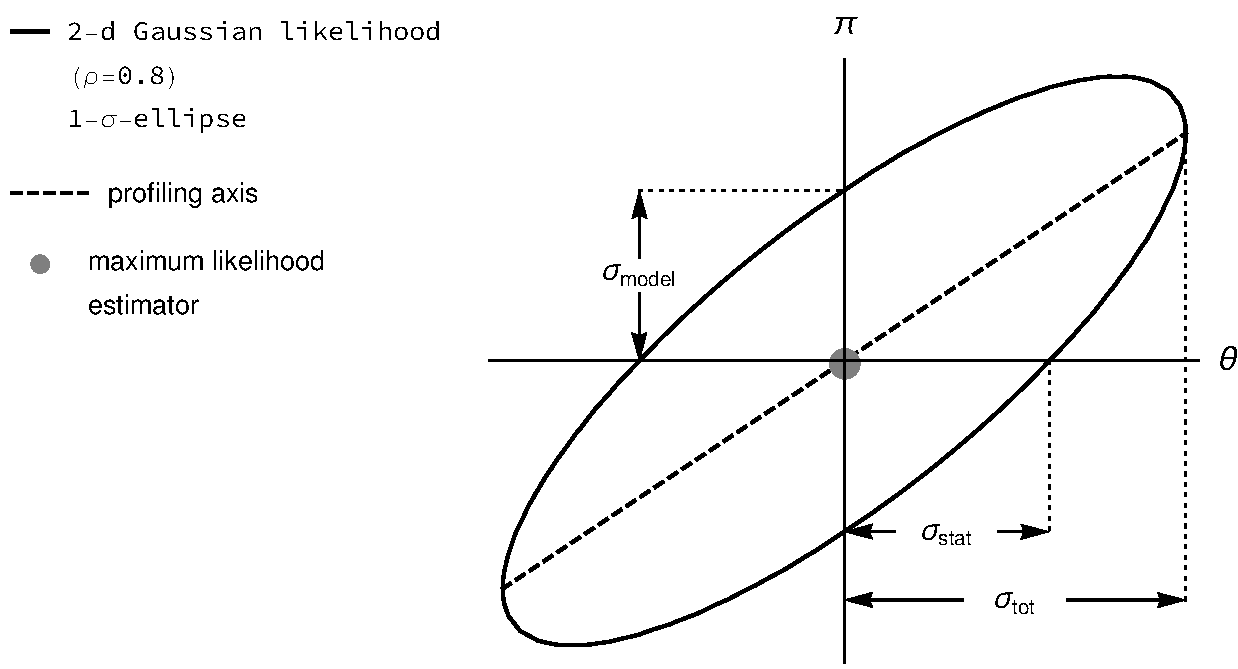
\includegraphics[width=\textwidth]{\currentFigureFolder/profileLikelihood.pdf}
	\xcaption{}{}{}
	\label{fig:katrinElossStatisticsProfileLikelihood}
\end{figure}
Apart from the  parameters of interest $\paramVec$ (usually the squared neutrino mass), the KATRIN likelihood depends on further so-called nuisance parameters $\nuisanceParamVec$ (e.\,g. the background rate). The dimensionality may pose difficulties when deriving a confidence region for the combined parameter set. Furthermore, as indicated by the naming conventions, the dimensions of the nuisance parameters in the confidence region are not of interest. Hence, in order to derive a confidence interval with restricted dimensions, a test statistic, similar to the one in equation~\ref{eq:statMethodsLikelihoodRatio}, but that solely depends on the parameters of interest, has to be found. The following paragraph outlines, how a corresponding test statistic can be constructed using the profile likelihood method.

A corresponding derivation may start with the definition of the profile likelihood: The profile likelihood only depends on the parameters of interest $\paramVec$. Its values correspond the likelihood values evaluated at $\paramVec$ in the dimensions of the parameters of interest and maximized in the dimensions of the nuisance parameters~\cite{ReviewOfParticlePhysics}
\begin{equation}
\profLikelihood(\paramVec) = 
L(\paramVec, \hat{\hat{\nuisanceParamVec}}(\paramVec))
\comma
\end{equation}
where the double-hat indicates the maximization respectively the profiling. Also, the profile likelihood ratio can be defined~\cite{ReviewOfParticlePhysics}
\begin{equation}
\label{eq:statMethodsProfileLikelihoodRatio}
\lambda_\mathrm{p}(\paramVec) = 
\frac{\profLikelihood(\paramVec)}{\profLikelihood(\hat{\paramVec})}
\fullstop
\end{equation}
According to Wilks’ theorem~\cite{wilks1938}, the distribution of $-2\ln\lambda_\mathrm{p}(\hat{\paramVec})$, where $\hat{\paramVec}$ is the \gls{mle}, approaches a $\chi^2$ distribution in the limit of a large data sample, independent of the values of the nuisance parameters $\nuisanceParamVec$~\cite{ReviewOfParticlePhysics}. Hence, the profile likelihood ratio offers a test statistic, from which a confidence interval for the parameters of interest can be derived.

In application to a KATRIN neutrino mass measurement, the introduced formalism can be summarized as follows: The profile likelihood~\eqref{eq:statMethodsProfileLikelihoodRatio} is a measure (test statistic) for whether a hypothesized squared neutrino mass has to be rejected given the KATRIN data. Furthermore, analogously to section~\ref{sec:statMethodsUncertaintyIntervalsConfidence}, this allows for the derivation of a confidence interval for the squared neutrino mass. It should be noted, however, that this method requires an extrapolation of the likelihood to nonphysical negative squared neutrino masses~\cite{Kleesiek2014}.

\subsection{Extension of the KaFit Software Framework}
\label{sec:katrinElossStatisticsImplementation}
The likelihood $L(\paramVec)$ can be multiplied by a function $g(\paramVec)$
\begin{equation}
\label{eq:likelihoodExtension}
-2\ln L^\prime(\paramVec) = -2\ln L(\paramVec) -2\ln g(\paramVec)
\fullstop
\end{equation}
This procedure may have different interpretations and usage scenarios. E.g. a comparison with \eqref{eq:posterior} shows, if $g$ is a prior probability distribution, $L^\prime$ becomes a non-normalized posterior distribution that can be used in a Bayesian analysis. A further interpretation is given in section \ref{sec:combinationOfMeasurements}.
\label{sec:combinationOfMeasurements}

KaFit allowed to choose $g$ in \ref{eq:likelihoodExtension} as a product of one-dimensional Gaussian distributions. Within this thesis the software was extended to allow products of other functions. Three function types were explicitly made available through a configuration file.
\begin{enumerate}
	\item A reimplementation of a one-dimensional Gaussian distribution: The reimplementation was necessary to conveniently enable the combination of function types.
	\item A multivariate Gaussian distribution: This enables the treatment of uncertainties quantified by calibration or monitor measurements as described in section \ref{sec:combinationOfMeasurements}. It can also be used as a prior distribution in a Bayesian analysis. Particularly, correlations can be respected.
	\item A one-dimensional probability density, that is constant in the square root of a parameter, if it is positive and 0 otherwise:
	\begin{equation}
		g(\theta) =
		\begin{cases}
		0 &\text{ if } \theta \leq 0 \\
		\text{constant} \cdot \frac{1}{\sqrt{\theta}} &\text{ if } \theta > 0
		\end{cases}
		\fullstop
	\end{equation}
	 This can be used as a uniform prior on the neutrino mass ($\theta=m_\nu^2$). Formerly, it was only possible to use a uniform prior on the squared neutrino mass. A derivation of the form of $g$ can be found in appendix \ref{sec:appStatisticPriorOnNu2}.
\end{enumerate}
An example on how to configure KaFit using the new feature is given in appendix \todo{Add appendix}.
